\documentclass[a4paper, 12pt]{scrartcl}

% Most of the preamble is in here.
\usepackage{atureport}

% Heading
\title{Individual Project: Denoising data signal with Fast Fourier Transform using Python coding}
\author{Abdul Fatah Jamro \\
 \\ID: G00425616}
\date{\today}


\begin{document}
  
\maketitle
 
\tableofcontents

\newpage

\section{Introduction}


Noise in the data has remained a major concern for scientists and engineers.
Various techniques are used like shields to protect or avoid noise, as well as denoising techniques.
Till now, Fast Fourier Transform (FFT) has remained on of the best approach to denoise, compress or analyse the data.
In the field of signal processing, noise removal is a basic issue which is tackled FFT.
It gets a lot easier when FFT is done with the help of computing tools.
In this study Python is used as tool to apply Fast Fourier transform in denoising a noisy audio signal.
Following sections briefly explain Fourier series, Fourier transform, and Fast Fourier transform, followed by example coding in Python. 

\subsection{Fourier Series}
A wave form or any periodic function is represented as a Fourier series, which is the sum of sines and cosines.
It bears the name Jean-Baptiste Joseph Fourier after the French mathematician and scientist (1768--1830).
Fourier transformations are frequently utilized in signal processing because sine waves are the building blocks of sound waves~\cite{tolstov1976fourier}.
Complex waves, like sound, can be said as a combination of sine waves using a Fourier series.
The series adds together the sines and cosines of a wave.

This implies that a wave's constituent parts can be separated from one another.
The study of various Fourier series falls within the category of Fourier analysis.
A Fourier transform is a technique for separating a signal into its various frequencies~\cite{tolstov1976fourier}.
Although a Fourier series can be calculated manually, computers are better able to decipher the intricate harmonics of commonplace sounds.
In audio processing, such as when isolating specific sounds from a recording, Fourier analysis is frequently utilized~\cite{tolstov1976fourier}.

\subsection{Fourier Transform}
The Fourier transform (FT) uses pattern based on time as its input to calculate the strength, rotation speed, and total cycle offset for each potential cycle.
Waveforms, having a function of time, space, or another variable, are subjected to the Fourier transform.
The Fourier transform represents any signal into sinusoid form.

A time function waveform is broken down into its constituent frequency function using the Fourier transform mathematical function.
The Fourier transform generates a complex valued function of frequency as its output.
While the Fourier transform's complex argument indicates the phase offset of the fundamental sinusoidal in that frequency, its absolute value represents the frequency value present in the original function.

Fourier transform is referred as a generalization of the Fourier series.
FT can be used to describe both the mathematical operation used and the representation of the frequency domain.
With the help of FT, the Fourier series can also be applied to non-periodic signals

The Fourier Transform (FT) of a function $f(x)$ is:

\begin{equation}
  F(k) = \int^{\infty}_{-\infty} f(x) e^{-2 \pi i k x} \,dx
\end{equation}

and the inverse can be obtained using inverse Fourier transform:

\begin{equation}
  f(x) = \int^{\infty}_{-\infty} F(k) e^{2 \pi i k x} \,dk
\end{equation}

Some of the properties of Fourier transform are as follows.

\begin{description}
  \item[Linear transform:] If $g(t)$ and $h(t)$ are two Fourier transforms given by $G(f)$ and $H(f)$ respectively, then the Fourier transform of the linear combination of $g$ and $t$ can be easily calculated.
  \item[Time shift property:] The Fourier transform of $g(t - a)$ where a is a real number that shfts the original function has the same amount of shift in the magnitude of the spectrum.
  \item[Modulation property:] A function is modulated by another function when it is multiplied in time.
  \item[Parseval's theorem:] Fourier transform is unitary, i.e., the sum of square of a function $g(t)$ equals the sum of the square of its Fourier transform, $G(f)$.
  \item[Duality:] The Fourier transform of $G(t)$ is $g$ if $g(t)$ possesses the Fourier transform $G(f) (-f)$.
\end{description}


\section{Fast Fourier Transform (FFT)}

The discrete Fourier transform (DFT) is a tool to do some sorts of functions of sequences into some other kind of representations.
DFT is long computing method whereas FFT is fast and short, relatively.
A fast Fourier transform (FFT) algorithm calculates the discrete Fourier transform (DFT) of some sequence.

The discrete Fourier transform also converts a waveform's cycle structure into sine components, which is another way to explain it.
A Fast Fourier transform can be applied to many different signal processing techniques.
It might be helpful for image-processing technology or for reading things like sound waves.
A Fast Fourier transform can be used to quickly solve different kinds of equations or display different kinds of frequency activity.

Fast Fourier transform and the DFT, which are exceedingly technical aspects of both computing and electrical engineering, are mostly the domain of engineers and mathematicians attempting to alter or build components of various technologies.
For example, fast Fourier transform might be helpful in sound engineering, seismology or in voltage measurements.
The FFT is a crucial measurement technique in the study of measuring audio and acoustics.
It breaks down a signal into its distinct spectral components, giving frequency information about the signal in the process.

FFTs are used for machine or system condition monitoring, quality control, and fault analysis.
This page covers the operation of an FFT, the pertinent parameters, and how they affect the measurement outcome.
The FFT is efficient implementation of the DFT~\cite{FFT}

A signal is separated into its frequency components after being sampled over time.
Each of these elements is a discrete sinusoidal oscillation with a unique frequency, amplitude, and phase.
The figure that below shows the transformation.

The Fourier Transform is a potent tool for looking at data from the frequency domain, as unlike to the time domain.
With its mathematical formulas, this powerful process, however, appears frightening.
Transform time-domain wave to frequency-domain, where $N$ is the number of samples:

\begin{equation}
  X_k = \sum_{n=0}^{N-1} x_n e^{-2 \pi i k n / N}
\end{equation}

Data can be easily manipulated in frequency domain, like removing noise or applying data compression.
Then, we can reverse the frequency domain to time domain by reversing equation

\begin{equation}
  x_n = \sum_{k=0}^{N-1} X_k e^{2 \pi i k n / N}
\end{equation}

Figure \ref{fig:fourier} illustrates the Fourier Transform (FT): decomposition of a sophisticated wave into different sinusoidal waves.

\begin{figure}[H] 
  \centering
  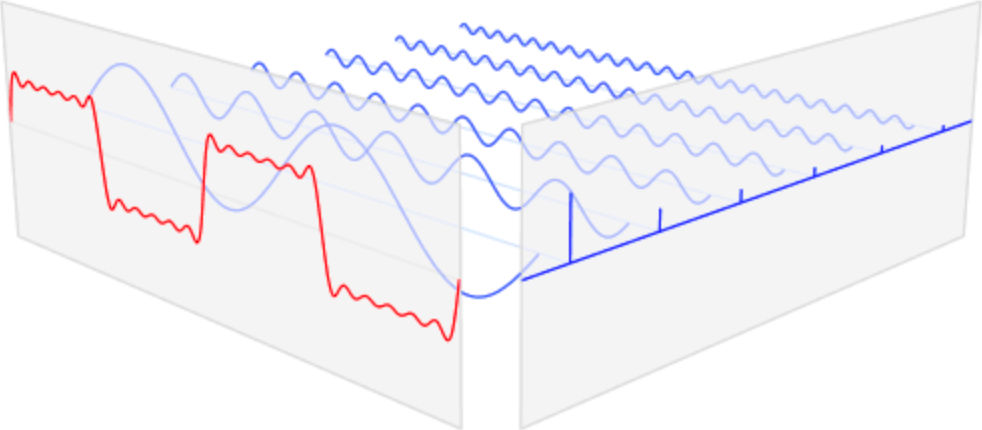
\includegraphics[width=0.6\textwidth]{img/fourier-dimensions.png}
  \caption{Frequency and time domains of a signal. (Image source wikipedia)}
  \label{fig:fourier}
\end{figure}

The wave function in red is the fourier sum of six other different waves shown in blue color. The Fourier Transform reveals the amplitudes summed sine waves.
 Each bar on right side of the image shows a different frequency.  

\section{Practical apllication of denoising audio signal}
Let us put aside for the time being the difficulty of FT equations.
Let us pretend that we fully get the meaning of the mathematical equations and apply the Fourier Transform to carry out some useful work in Python~\cite{CleanUpNoise}.

We create two audio signals of different frequencies with the help of python coding as shown in Figure~\ref{fig:sixty} and Figure~\ref{fig:onefifty} 
and convolute them into single resultant signal named clean signal as shown in the Figure~\ref{fig:sumsignals}. 
Both signals are the function of time-domain, their resultant and added noise are also the function of time-domain.
\subsection{Generating of two signals and their convolution sum with random noise}
\begin{figure}[H] 
  \centering
  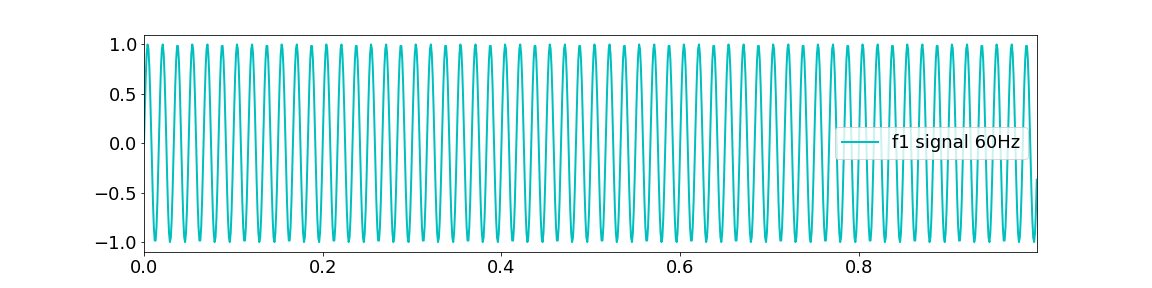
\includegraphics[width=\textwidth]{img/signal_60hz.png}
  \caption{A 60Hz signal.}
  \label{fig:sixty}
\end{figure}


\begin{figure}[H] 
  \centering
  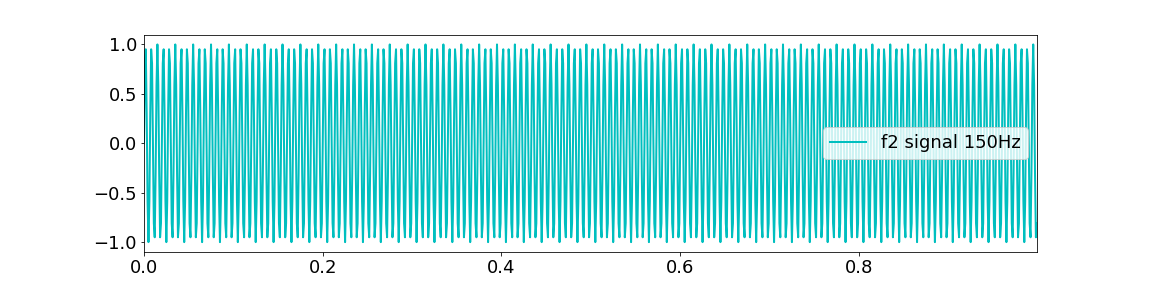
\includegraphics[width=\textwidth]{img/signal_150hz.png}
  \caption{A 150Hz signal.}
  \label{fig:onefifty}
\end{figure}

\begin{figure}[H] 
  \centering
  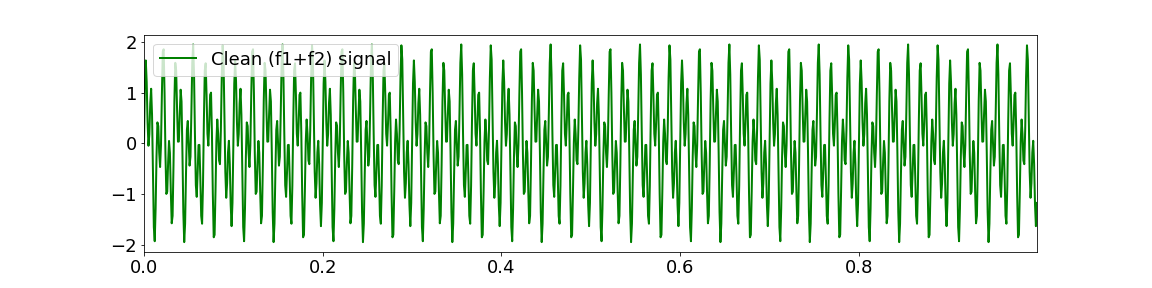
\includegraphics[width=\textwidth]{img/sum_signals.png}
  \caption{Sum of 60Hz and 150Hz signals.}
  \label{fig:sumsignals}
\end{figure}
\subsection{Adding some random noise to original signal}

Then, we deliberately created a random noise signal with random frequency and superimposed on our clean audio signal as in Figure~\ref{fig:original_noisy}. 
Figure~\ref{fig:time_to_freq} is the frequency-domain repesentation of Figure~\ref{fig:original_noisy}.

\begin{figure}[H] 
  \centering
  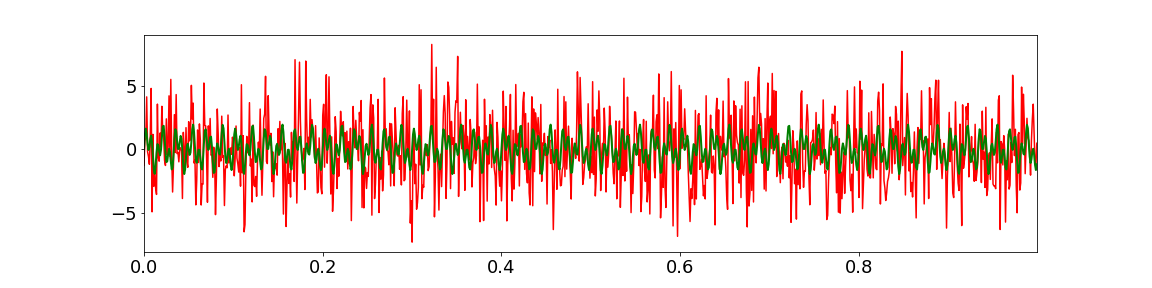
\includegraphics[width=\textwidth]{img/original_noisy.png}
  \caption{The noisy signal with original superimposed.}
  \label{fig:original_noisy}
\end{figure}

Figure~\ref{fig:sixty} to Figure~\ref{fig:original_noisy} are generated using the Python~\cite{fftnumpy} code in Listing~\ref{listing:sixty}

\begin{listing}[h]
  \begin{minted}{python}
 #importing libraries and setup
  import numpy as np
  import matplotlib.pyplot as plt
  dt = 0.001 # frame difference 0.001
  t = np.arange(0,1,dt) # time on x-axix
  f1 = np.sin(2*np.pi*60*t) #first signal f1 60Hz
  f2 = np.sin(2*np.pi*150*t) # second singal f2 150Hz
  f_clean= f1 + f2 # suming f1 and f2
  #add some random noise to the signal.
  f = f_clean + 2.5*np.random.randn(len(t))
  \end{minted}
  \caption{Code for time domin signals.}
  \label{listing:sixty}
  \end{listing}
  
\subsection{Converting time domain signal to frequency domain}

  In Figure~\ref{fig:time_to_freq}, is the noisy audio signal that needs to be filtered-out of noise.
Here is the use of Fast Fourier Transform (FFT) to filter out the noise and get original signal back.
  
\begin{figure}[H] 
  \centering
  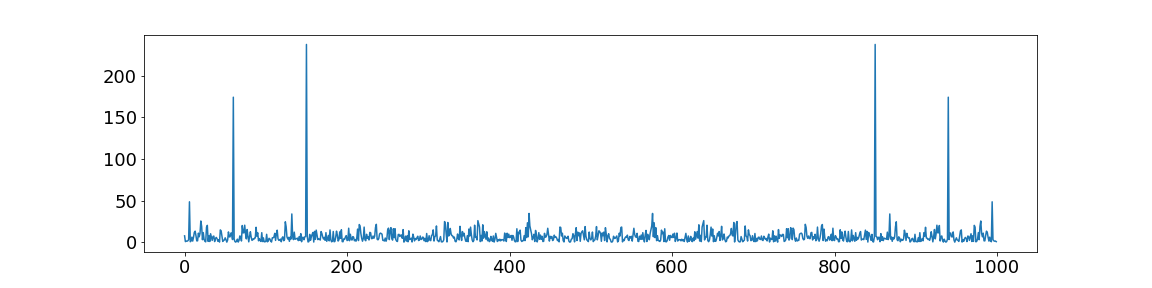
\includegraphics[width=\textwidth]{img/time_to_freq.png}
  \caption{The Frequency domain of the noisy signal.}
  \label{fig:time_to_freq}
\end{figure}
Initially, the time domain signal is changed into frequency domain using algorithm we already discussed of; FFT algorithm.
With the help of Fourier Transform it becomes easier to track frequencies and break signal into different frequencies.
FFT algorithm is the efficient way to do that job.

\begin{listing}[h]
  \begin{minted}{python}
  # Compute the Fast Fourier Transform (FFT)
  n = len(t)
  fhat = np.fft.fft(f,n)                     # Compute the FFT
  PSD = fhat * np.conj(fhat) / n             # Power spectrum density (power per freq)
  freq = (1/(dt*n)) * np.arange(n)           # Create x-axis of frequencies in Hz
  L = np.arange(1,np.floor(n/2),dtype='int') # Only plot the first half of freqs
  \end{minted}
  \caption{Coverting time domain to frequency domian with FFT algorithm.}
  \label{listing:time_to_freq}
  \end{listing}

  \subsection{Removing Noise by applying threshold}

  This is the frequency domain signal where each spike represents a different frequency signal, 
  It is easier to apply threshold to get rid of undesired signals~\cite{fftfilter}.  
  If we pick the frequencies that cross the index of 120 in y-axis, 
  we can omit 99percent noise because the noise indices are very low. 
  After applying the threshold of 120 we get the following signal, 
  which is totally free from noise, as shown in the Figure~\ref{fig:denoise_freq}. 
  It is still in frequency domain and can be converted back into time domain by doing inverse function of Fast Fourier Transform (IFFT)
  \begin{figure}[H] 
    \centering
    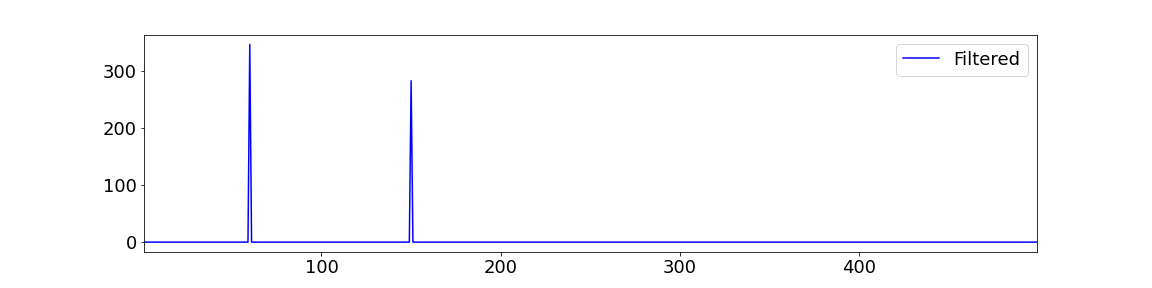
\includegraphics[width=\textwidth]{img/denoise_freq.png}
    \caption{The Frequency domain of the denoised signal.}
    \label{fig:denoise_freq}
  \end{figure}
  
  \begin{listing}[H]
    \begin{minted}{python}
    # Use the PSD (power spectral density) to filter out noise
    indices = PSD > 120       # Find all freqs with large power
    PSDclean = PSD * indices  # Zero out all others
    fhat = indices * fhat     # Zero out small Fourier coeffs. in Y
    ffilt = np.fft.ifft(fhat) # Inverse FFT for filtered time signal
    \end{minted}
    \caption{Noise removed in frequency domian by apply threshold PSD above 120 and inverse FFT.}
    \label{listing:denoise_freq}
    \end{listing}
  \subsection{Reversing the frequency domian signal to time domain}

    When we apply inverse FFT, we get signal in time domain which is almost identical to original convoluted summed signal 'f'.
Looking at the fig.09, we can see the green signal that is original convolution of two signals f1 and f2. 
The signal in blue is the filtered or recovered signal by removing noise. If both signals are compared there is not any difference and the information in signal is not lost. 
The filtered signal is almost alike the original signal 
\begin{figure}[H] 
  \centering
  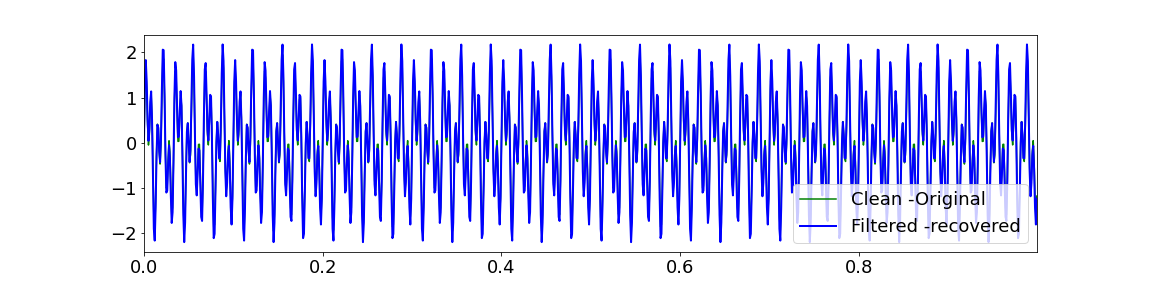
\includegraphics[width=\textwidth]{img/fft_infft_signals.png}
  \caption{Inverse FFT to covert back from frequency to time domain.}
  \label{fig:fft_infft_signals}
\end{figure}

\section{Conculsion}
We briefly, provided overview of fourier series, fourier transform and fast fourier transform (FFT). 
After that, we explained FFT algorithm for a practical application of denoising the data signal. Taking the advantage of Python programing tool, we generated two different signals then added some random noise to it.
then we proved with help of FFT and inverse FFT that the noise can be removed from data signals.\\
FFT algorithm is the one of the best algorithm till today~\cite{fftalg}. 
It is used in multiple problem solving approaches, like data cleaning, data analysing, data compression, analog and digital signal processing. It can also be used for mathematical modelling of PDEs and ODEs systems.
Quantum Mechanics and Quantum Computing fields can make use of FFT algorithm at larger scale.

    \newpage
\bibliographystyle{IEEEtran}
\bibliography{bibliography}
  
\end{document}